\documentclass[10pt,a4paper]{article}
\usepackage[utf8]{inputenc}

% Define the page margin
\usepackage[margin=3cm]{geometry}

% Better typography (font rendering)
\usepackage{microtype}

% Math environments and macros
\usepackage{amsmath}
\usepackage{amsfonts}
\usepackage{amssymb}
\usepackage{amsthm}

% Define \includegraphics to include graphics
\usepackage{graphicx}

% Draw graphics from a text description
\usepackage{tikz}

% Syntax highlighting
\usepackage{minted}

% Set global minted options
\setminted{linenos, autogobble, frame=lines, framesep=2mm}

\title{Operating Systems, Sheet 3}
\author{Marten Lienen (03670270)}

\begin{document}

\maketitle

\section*{Exercise 1}

\begin{itemize}
\item Array of 7 pointers to pointer of long
\item Some array of function pointers
\end{itemize}

\section*{Exercise 2}

\subsection*{Part 2.1)}

\begin{minted}{asm}
  A:
  sub a, b

  B:
  add c, d

  C:
  sub e, f

  D:
  sub a, b
  add c, d
  sub e, f
  mul a, c
  div a, e

  E:
  add v, w
  div u, v
  sub r, t
  mul u, r
  add q, p
  mul u, q
  div u, h
\end{minted}

\subsection*{Part 2.2)}

\begin{minted}{asm}
  D:
  concurrent {
    sub a, b
    add c, d
    sub e, f
  }

  mul a, c
  div a, e

  E:
  concurrent {
    add v, w
    sub r, t
    add q, p
  }

  concurrent {
    div u, v
    div q, h
  }

  mul u, r
  mul u, q
\end{minted}

\subsection*{Part 2.3)}

\subsection*{Part 2.4)}

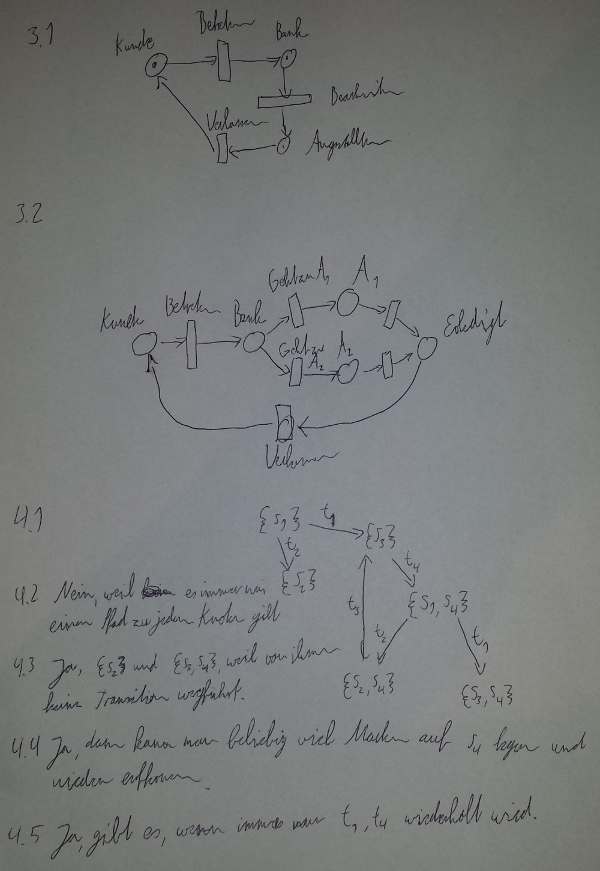
\includegraphics[width=450pt]{sheet-3/4}

\section*{Exercise 5}

\subsection*{Part 5.1)}

Nein, weil sie warten, wenn der Puffer leer bzw. voll ist.
Er kann aber nicht geleert bzw. gefüllt werden, weil der jeweils andere vom Semaphor daran gehindert wird.

\subsection*{Part 5.2)}

Man fügt jeweils einen Semaphor ein, der prüft, ob der Puffer leer ist, und einen, der prüft, ob der Puffer voll ist.

\subsection*{Part 5.3)}

Wenn man die Semaphoren in unterschiedlicher Reihenfolge lockt, kann es zum Deadlock kommen.

\end{document}
